% components.tex
%
% written 2022 by Werner Lemberg <wl@gnu.org>


% This file contains graphics used for the 'FreeType Design' documentation,
% part 1, 'Components and APIs'.


% Here is one possibility to convert this LaTeX file to both PNG and SVG
% formats.
%
%   xelatex components.tex
%
%   pdftoppm -png -f 1 -l 2 -r 120 components.pdf components
%   optipng components-*.png
%
%   for i in 1 2; do
%     pdf2svg components.pdf components-$i.svg $i
%   done


\documentclass[tikz,
               svgnames, % for xcolor
               border=3mm]{standalone}

\usepackage{libertinus}

\usetikzlibrary{
  calc,
  decorations.pathreplacing, % for "show path construction"
  fit,
  positioning,
  shapes.geometric
}


% Node styles.
\tikzset{
  % 'Elastic dashes' adapt spaces between dashes to the line length so that
  % the last dash doesn't get cut off partially.
  %
  % Taken from https://github.com/pgf-tikz/pgf/issues/629
  elastic dashes/.code args={on #1 off #2 ends #3}{%
    % Use csname so catcode of @ doesn't have do be changed.
    \csname tikz@addoption\endcsname{
      \pgfgetpath\currentpath
      \pgfprocessround{\currentpath}{\currentpath}
      \csname pgf@decorate@parsesoftpath\endcsname
        {\currentpath}{\currentpath}
%
      \pgfmathparse{max(#1 - #3, 0)}
      \let\dashphase=\pgfmathresult
      \pgfmathparse{\csname pgf@decorate@totalpathlength\endcsname
                    - #1
                    + 2 * \dashphase}
      \let\rest=\pgfmathresult
      \pgfmathparse{#1 + #2}
      \let\onoff=\pgfmathresult
      \pgfmathparse{max(floor(\rest / \onoff), 1)}
      \let\nfullonoff=\pgfmathresult
      \pgfmathparse{max((\rest - \onoff * \nfullonoff) / \nfullonoff + #2,
                        #2)}
      \let\offexpand=\pgfmathresult
%
      \pgfsetdash{{#1}{\offexpand}}{\dashphase pt}}
  },
%
  % Elastic dashes for boxes and the like.
  elastic dashes per segment/.style args={on #1 off #2 ends #3}{
    /utils/exec=\csname tikz@options\endcsname,
    decoration={
      show path construction,
      lineto code={
        \draw [elastic dashes=on #1 off #2 ends #3]
          (\tikzinputsegmentfirst)
          -- (\tikzinputsegmentlast);},
      curveto code={
        \draw [elastic dashes=on #1 off #2 ends #3]
          (\tikzinputsegmentfirst)
          .. controls (\tikzinputsegmentsupporta)
             and (\tikzinputsegmentsupportb)
          .. (\tikzinputsegmentlast);},
      closepath code={
        \draw [elastic dashes=on #1 off #2 ends #3]
          (\tikzinputsegmentfirst)
          -- (\tikzinputsegmentlast);}},
    decorate},
%
  % The distance between 'module' nodes.
  node distance=0.3cm,
%
  % For normal lines.
  line/.style={
    line width=1pt},
%
  % For thin lines.
  thin line/.style={
    line width=0.5pt},
%
  % For arrow lines.
  arrow line/.style={
    thin line,
    -latex},
%
  % For boxes in general.
  box/.style={
    line,
    draw,
    minimum height=1cm,
    line cap=rect},
%
  % For base components.
  base box/.style={
    box,
    minimum width=1.5cm,
    minimum height=0.5cm,
  },
%
  % For optional base components.
  optional base box/.style={
    base box,
    elastic dashes per segment=on 3pt off 3pt ends 2pt
  },
%
  % For module boxes.
  module box/.style={
    box,
    outer sep=0pt,
    minimum width=1.8cm},
%
  % For service boxes.
  service box/.style={
    thin line,
    draw,
    outer sep=0pt,
    anchor=south west,
    font=\tiny},
%
  % Generic triangles.
  triangle/.style={
    thin line,
    isosceles triangle,
    isosceles triangle stretches,
    inner sep=0pt,
    minimum width=0.25cm,
    minimum height=0.2cm,
    draw},
%
  % For triangles pointing upwards.
  triangle up/.style={
    triangle,
    shape border rotate=90,
    fill=#1},
%
  % For triangles pointing downwards.
  triangle down/.style={
    triangle,
    shape border rotate=-90,
    fill=#1},
%
  % For triangle descriptions.
  triangle description/.style args={#1/#2}{
    triangle down=#1,
    label={[label position=south,
            anchor=base west]:\ #2}},
%
  % We use a 'matrix' as a means to get a pre-computed bounding box node of
  % a group of nodes.
  %
  % In particular, we use matrices to center two rows of boxes both
  % horizontally (i.e., to align the center the first row of boxes with the
  % center of the second row).
  container/.style={
    matrix,
    every outer matrix/.style={
      inner sep=0pt,
      outer sep=0pt}}
}


% Locations on top or bottom edges of boxes.
\def\pos#1#2{($ (#1 west) !#2! (#1 east) $)}


%%%%%%%%%%%%%%%%%%%%%%%%%%%%%%%%%%%%%%%%%%%%%%%%%%%%%%%%%%%%%%%%%%%%%%%%%%%%%

\begin{document}

% Basic library design.

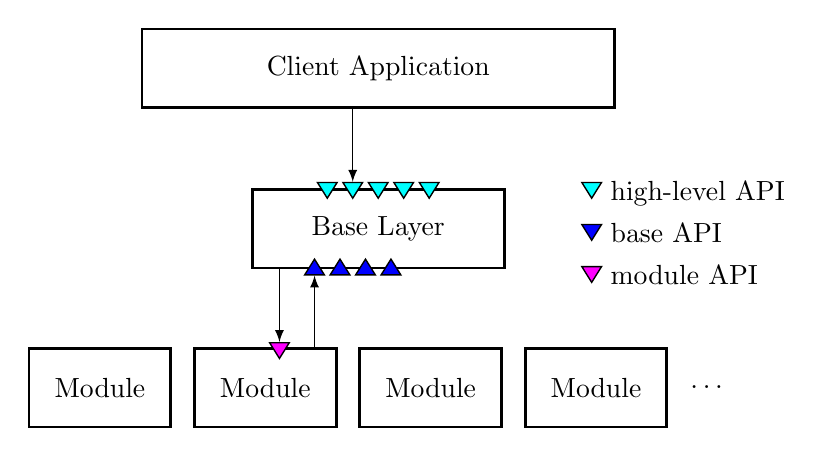
\begin{tikzpicture}
  \node[module box] (M1) {Module};
  \foreach \x [remember=\x as \lastx (initially 1)] in {2, 3, 4}
    \node[module box] (M\x) [right=of M\lastx] {Module};
  \node[inner sep=0pt,
        outer sep=0pt] (Mdots) [right=of M4] {\ldots};

  \node[inner sep=0pt,
        outer sep=0pt,
        fit=(M1) (Mdots)] (Mboxes) {};
  \node[box,
        minimum width=3.2cm] (B) [above=1cm of Mboxes]
       {Base Layer};
  \node[box,
        minimum width=6cm] (C) [above=1cm of B]
       {Client Application};

  \foreach \i/\x in {1/0.3, 2/0.4, 3/0.5, 4/0.6, 5/0.7}
    \node[triangle down=Aqua] (Btop\i) at \pos{B.north}{\x} {};
  \draw[arrow line] (C.south -| Btop2) -- (Btop2);

  \foreach \i/\x in {1/0.25, 2/0.35, 2/0.45, 3/0.55}
    \node[triangle up=Blue] (Bbottom\i) at \pos{B.south}{\x} {};
  \draw[arrow line] (M2.north -| Bbottom1) -- (Bbottom1);

  \node[triangle down=Fuchsia] (M2top) at \pos{M2.north}{0.6} {};
  \draw[arrow line] (B.south -| M2top) -- (M2top);

  \node[triangle description=Aqua/high-level API] (T1)
    [right=1cm of B.north east] {};
  \node[triangle description=Blue/base API] (T2) [below=2ex of T1] {};
  \node[triangle description=Fuchsia/module API] (T3) [below=2ex of T2] {};
\end{tikzpicture}


% Detailed library design.

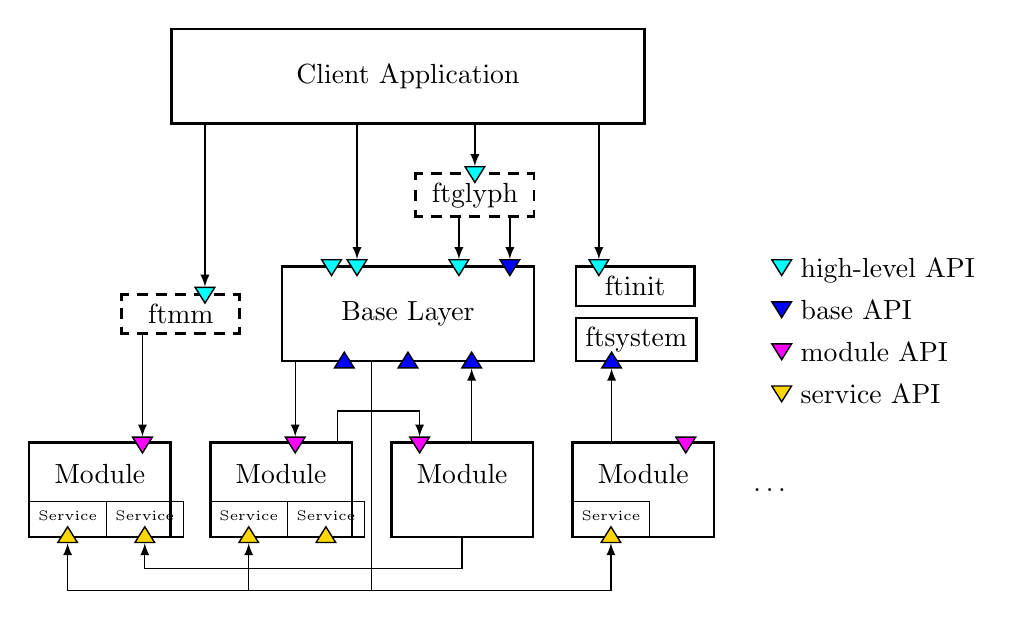
\begin{tikzpicture}
      [node distance=0.5cm,
       box/.append style={
         minimum height=1.2cm},
       module box/.append style={
        text depth=0.4cm},
       service box/.append style={
        text depth=0.1cm}]
  \node[container] (module boxes) {
    \node[module box] (M1) {Module};
    \foreach \x [remember=\x as \lastx (initially 1)] in {2, 3, 4}
      \node[module box,
            right=of M\lastx] (M\x) {Module};
    \node[inner sep=0pt,
          outer sep=0pt,
          right=of M4] (Mdots) {\ldots};

    \node[service box] (S1A) at (M1.south west) {Service};
    \node[service box] (S1B) at (S1A.south east) {Service};
    \node[service box] (S2A) at (M2.south west) {Service};
    \node[service box] (S2B) at (S2A.south east) {Service};
    \node[service box] (S4A) at (M4.south west) {Service};
    \\
  };

  \node[container,
        above=1cm of module boxes] (base boxes) {
    \node[box,
          minimum width=3.2cm] (B) {Base Layer};
    \node[base box,
          right=of B.north east,
          anchor=north west] (FI) {ftinit};
    \node[base box,
          right=of B.south east,
          anchor=south west] (FS) {ftsystem};
    \node[optional base box,
          left=of B] (FM) {ftmm};
    \\
  };

  \node[optional base box,
        above=0.6cm of B.north east,
        anchor=south east] (FG) {ftglyph};

  \coordinate[above=0.6cm of FG] (c);
  \node[box,
        minimum width=6cm,
        anchor=south] (C) at (B |- c) {Client Application};

  \node[triangle down=Aqua] (FMtop) at \pos{FM.north}{0.7} {};
  \node[triangle down=Aqua] (FGtop) at \pos{FG.north}{0.5} {};
  \node[triangle down=Aqua] (Btop1) at \pos{B.north}{0.2} {};
  \node[triangle down=Aqua] (Btop2) at \pos{B.north}{0.3} {};
  \node[triangle down=Aqua] (Btop3) at \pos{B.north}{0.7} {};
  \node[triangle down=Blue] (Btop4) at \pos{B.north}{0.9} {};
  \node[triangle up=Blue] (Bbottom1) at \pos{B.south}{0.25} {};
  \node[triangle up=Blue] (Bbottom2) at \pos{B.south}{0.50} {};
  \node[triangle up=Blue] (Bbottom3) at \pos{B.south}{0.75} {};
  \node[triangle down=Aqua] (FItop) at \pos{FI.north}{0.2} {};
  \node[triangle up=Blue] (FSbottom) at \pos{FS.south}{0.3} {};
  \node[triangle down=Fuchsia] (M1top) at \pos{M1.north}{0.8} {};
  \node[triangle down=Fuchsia] (M2top) at \pos{M2.north}{0.6} {};
  \node[triangle down=Fuchsia] (M3top) at \pos{M3.north}{0.2} {};
  \node[triangle down=Fuchsia] (M4top) at \pos{M4.north}{0.8} {};

  \foreach \x in {S1A, S1B, S2A, S2B, S4A}
    \node[triangle up=Gold] (\x bottom) at (\x.south) {};

  \draw[arrow line] (C.south -| FMtop) -- (FMtop);
  \draw[arrow line] (C.south -| Btop2) -- (Btop2);
  \draw[arrow line] (FG.south -| Btop3) -- (Btop3);
  \draw[arrow line] (FG.south -| Btop4) -- (Btop4);
  \draw[arrow line] (M3.north -| Bbottom3) -- (Bbottom3);
  \draw[arrow line] (C.south -| FGtop) -- (FGtop);
  \draw[arrow line] (C.south -| FItop) -- (FItop);
  \draw[arrow line] (M4.north -| FSbottom) -- (FSbottom);
  \draw[arrow line] (FM.south -| M1top) -- (M1top);
  \draw[arrow line] (B.south -| M2top) -- (M2top);
  \draw[arrow line] \pos{M2.north}{0.9} -- +(0,0.4) -| (M3top);

  \coordinate[below=0.6cm of S1Abottom] (m);
  \coordinate (mm) at ($ (M2) !0.5! (M3) $);
  \draw[thin line] (B.south -| mm) -- (m -| mm);
  \draw[thin line] (S1Abottom |- m) -- (S4Abottom |- m);
  \draw[arrow line] (S1Abottom |- m) -- (S1Abottom);
  \draw[arrow line] (S2Abottom |- m) -- (S2Abottom);
  \draw[arrow line] (S4Abottom |- m) -- (S4Abottom);

  \draw[arrow line] (M3.south) -- +(0,-0.4) -| (S1Bbottom);

  \node[triangle description=Aqua/high-level API,
        right=1cm of FI.north east] (T1) {};
  \node[triangle description=Blue/base API,
        below=2ex of T1] (T2) {};
  \node[triangle description=Fuchsia/module API,
        below=2ex of T2] (T3) {};
  \node[triangle description=Gold/service API,
        below=2ex of T3] (T4) {};
\end{tikzpicture}

\end{document}
